\documentclass[preprint,aip,jap]{revtex4-2}

\usepackage[latin9]{inputenc}
\usepackage{graphicx}
\begin{document}
\title{Molecular alignment at graphene surface determines tansport properties of graphene transistors}

\author{Vadym Tkachuk}%
\author{Egon Pavlica}%
\author{Gvido Bratina}%
\altaffiliation[Corresponding author. E-mail:]{\tt{bratina@ung.si}}
\affiliation{Laboratory for Organic matter physics,University of Nova Gorica,\\
  Vipavska 13, SI-5000 Nova Gorica, Slovenia}%
\date{\today}

\begin{abstract}

  Graphene field-effect transistor structures were used to investigate the role of molecular alignment on charge transport properties of heterostructures comprising a single-layer graphene and variable thickness of N,N'-bis(n-octyl)-(1,7\&1,6)-dicyanoperylene-3,4:9,10-bisdicarboximide (PDI8-CN2) - an n-type organic semiconductor. Our atomic force microscopy data show that under selected growth conditions PDI8-CN2 grows in a layer-by-layer fashion up to a second monolayer. The first layer comprises flat-lying molecules, whereas the molecules in the second layer orient themselves in an upright orientation. Transconductance measurements show that the flat-lying molecules have little effect on the position of the Fermi level in graphene. Upright oriented molecules in the second layer instead have a strong effect as to neutralize native $p$-type doping of graphene and cause a shift of charge-neutrality level towards the Dirac point. We interpret such behavior in terms of different orientation of the surface dipole on layers with different molecular orientations. At the same time the overall mobility of the charge carriers reaches values exceeding 3000 cm$^{2}$/Vs.  
\end{abstract}

\keywords{graphene, atomic force microscopy, charge transport, organic semiconductors}

\maketitle

\section{\label{sec:intro}Introduction}

One of the venue to improve switching and optical capabilities of graphene in potential high-speed electronic applications\cite{novoselov-2004} or photodetectors includes coupling with organic semiconductors (OS). In this regard  two basic approaches are most common. Blending of graphene nanoflakes with OS  has been demonstrated to effective both in polymer OS\cite{pathipati-2015,elgemayel-2014,liscio-2011} or small-molecule OS \cite{pathipati-2014}. The other approach includes interfacing graphene with OS overlayers\cite{pathipati-2019,pathipati-2015,huisman-2015,kim-2017b,ha-2012,zhou-2013a,nouchi-2008,nouchi-2014}. Charge transport in blends can be described in terms of combination of hopping through the manifold of localized states on OS molecules and extended-state transport on graphene. Less clear is the situation in the case of OS overlayers on graphene, especially when the OS layer thickness remains in the range of few molecular layers. In this case, the electric field due to the charge imbalance on the molecules may still have an important effect on the position of the Fermi level in graphene. Most of the published experiments including those presented here include mechanically exfoliated graphene flakes transferred onto SiO$_{2}$ in air. The resulting redox reactions at the substrate surface cause $p$-type doping of graphene \cite{feng-2014,peng-2017,lafkioti-2010}, which may be changed upon deposition of OS molecules either via charge transfer or dipole/multipole-induced charge accumulation at the interface. This inevitably alters charge-transporting properties of the final graphene/OS system, and must be considered when interpreting current-voltage ($I-V$) characteristics of graphene field-effect-transistors (GFETs) that include thin OS overlayers. 

Research in initial stages of growth of OS on dielectric substrates is plentiful and a thorough review of the subject is beyond the scope of this article. It is important to note, however that initial stages of growth of OS are extremely sensitive to all three relevant parameters: arriving rate of the molecules, their surface mobility and the rate of island nucleation. The work by Ruiz et al. \cite{ruiz-2004}, for example, summarizes rich morphology that can be achieved by altering growth conditions of pentacene on SiO$_{2}$. Similar findings hold for other small-molecule OSs as well as polymers grown from the solution. The importance of the ability to control the initial stages of growth can't be overemphasized, since it is in this stage that the morphology of thicker layer is determined, and the coupling between the layer morphology and its charge transport properties are well known.

As for the graphene-based electronic devices initial stages of growth are particularly important since in this stage the orientation of molecules on the substrate are determined. The geometrical orientation of the electric dipoles and multipoles depends, in turn on the orientation of the molecule on the substrate\cite{geng-2012}. The electric field dipole exhibits a $\propto 1/r^{3}$ dependence on the distance from the dipole and is thus important only for the extremely thin overlayes on graphene. In addition it is important that the overlayers are structurally coherent i.e. monocrystalline domains are as large as possible in order to reduce disorder-related reduction in the effects of surface dipoles. Indeed, as  we show in this work, charge carrier transport in such material systems is crucially dependent on the molecular orientation at the graphene/OS interface. For this type of research it is important to select OS that exhibits high charge carrier mobility per se, in order to preserve high mobility on graphene.   N,N'-bis(n-octyl)-(1,7\&1,6)-dicyanoperylene-3,4:9,10-bisdicarboximide (PDI8-CN2)
 exhibits a remarkable air stability, solution processability and relatively high electron mobility in thin film form\cite{jung-2014,molinari-2009,piliego-2009a}.  The position of the lowest unoccupied molecular orbital (LUMO) in this material is at 7.1 eV\cite{jung-2014}, which makes it suitable for interfacing with graphene, whose Dirac point is at $~4.5$ eV.

Our results show that under the selected growth conditions PDI8-CN2 forms well ordered layers up to the second layer. The growth mode is rather complex since the molecules are oriented flat on the graphene surface in the first layer. In the second layer the molecules are oriented almost perpendicular to the surface. This has profound consequences on the measured transfer characteristics. Due to the orientation of the surface dipole of the molecules in the first layer, its effect on the transport properties of graphene is almost negligible, and transfer characteristics of the clean graphene relative to that of the 70\% covered with PDI8-CN2 are very similar. On the other hand when the second PDI8-CN2 layer is completed its surface dipole causes a major effect on the position of the charge neutrality level in graphene so that it almost coincides with the position of the Dirac point.  The overall mobility of the structure is reduced relative to the clean graphene, albeit reaches values higher than 3400 cm$^{2}$/Vs, which is a remarkable value for the OS/graphene system. 





\section{\label{sec:exper}Experimental methods}


Graphene was obtained by mechanical exfoliation of highly oriented pyrolytic graphite. Subsequently graphene flakes were transferred onto p-doped silicon wafers covered with 285 nm-thick thermally grown oxide layer. Onto such surface PDI8-CN2 layers were fabricated by Organic Molecular Beam Epitaxy in a vacuum chamber with the base pressure of $1\times10^{-8}$ mbar. PDI8-CN2 powder without any further purification, was used as a source material. The temperature of the substrate during organic semiconductor (OS) growth was 45$^\circ$C. Samples with three different PDI8-CN2 coverages were examined. The coverage variation was achieved by varying the growth time, which comprised 1, 3 and 4 minutes. The thickness of graphene flakes and the morphology of PDI8-CN2 layers were examined using an optical microscope and an Atomic Force Microscope (AFM) operating in non-contact mode in air. Data analysis was performed with Gwyddion software\cite{necas-2012}. The $I-V$ characteristics measurements of GFETs were performed by using a Keithley 6487 Picoammeter/Voltage Supply and a Keithley 2400 SorceMeter. Drain current ($I_{DS}$) was measured by varying the gate voltage ($V_G$) in the range from -50 to +50 V at two values of the source-drain bias: 0.001 and 0.01 V. All measurements were performed in a nitrogen-filled glovebox with H$_2$O and O$_2$ concentration of less than 10 ppm.  Carrier mobility was calculated from $I-V$ curves using the equation, where $L$ and $W$ are the dimensions of the conductive channel, d is the thickness of the silicon oxide layer. Each sample was measured before and after deposition of PDI8-CN2 on it.

\section{\label{sec:res}Results and Discussion}

\subsection{\label{sec:morph}Morphology}

Morphology of the PDI8-CN2 layer on a single layer graphene is shown in Figure \ref{fig:1}a, where we show a LxW $\mu m^2$ AFM topography scan of the area of the sample. The topography of graphene is flat and characterized by few linear steps/folds in the upper left part of the image. In the image brighter tones represent higher elevations, and the dark irregular patches represent depressions in the otherwise continuous PDI8-CN2 layer. Figure \ref{fig:1}b  shows a normalized distribution of the height data obtained from the image shown in Figure \ref{fig:1}a). The data (dark points) were fitted with two Gaussian functions (green curves) that yield a composite fit (red curve) for the whole range of data. The lower peak in the distribution corresponds to the height data from the depressions, and the higher peak corresponds to the data of the layer. The origin of the height scale has been shifted to the position of the centroid describing the depressions, so that the height difference between the centroids of the two Gaussian functions reads as 0.66$\pm$xx nm, where the error is the average of the full-width at half maximum of the two Gaussian functions.  The thickness of the PDI8-CN2 layer is therefore 0.664$\pm$ xx nm.\textbf{ *Continue*}
\begin{figure}[htb]
  \centering
        \includegraphics[width=0.9\textwidth]{./Figures/fig1}
  \caption{a) The non-contact topography map of the PDI8-CN2 layer on a single-layer graphene. The growth time was 1 minute. Brighter tones represent higher elevations. The straight lines in the upper left portion of the image are folds in graphene. Dark irregularly-shaped patches are depressions in an otherwise continuous layer of PDI8-CN2.  b) The height distribution of the image shown in Figure 1a). The histogram has been normalized to the highest value in the image. The black dots represent the data, the green curves are Gaussian functions used to fit the data. The composite fit is represented by the red curve. The leftmost peak corresponds to the depressions in the complete layer represented by the highest peak.}
  \label{fig:1}
\end{figure}

 
A detailed study of the initial stages of growth of PDI8-CN2 on SiO2 was studied by Liscio et al.\cite{liscio-2013}. They have compared the morphology of the layers grown at 25 $^\circ$C and at 120 $^\circ$C. Their results show that higher substrate temperature results at higher degree of order in the layers, which at 120 $^\circ$C grow predominantly by aggregation of molecules oriented almost perpendicularly to the substrate and yielding thickness of the first monolayer of ~1.8 nm. At 25 $^\circ$C instead they observe morphology that is characterized by a mixture of islands formed by molecules oriented upright on the substrate and the islands formed by molecules lying flat on the substrate (observed height ~0.5 nm). Interestingly, despite this heterogenous growth the surface roughness of the first monolayer is the same, albeit the layer density is lower in the samples prepared at room temperature, as assessed from the oscillations of the x-ray intensity. 


The observed layer thickness in our case is consistent with PDIF8-CN2 molecules lying flat on the graphene substrate, since the a-axis of the PDI8-CN2 unit cell, is 0.5 nm \textbf{[Ref]}. We also note, that no second layer nucleation is observed although the coverage of the first monolayer is 70 \%. This is consistent with the results from Ref. \onlinecite{liscio-2013}, who observed the onset of nucleation of the second layer upon completion of 95 \% coverage of the first. The rms roughness of our layers was consistently found to be XXX \%. As the exposure to the source materials increased from 1 minute to 3 minutes. The layer morphology changes as illustrated in Figure \ref{fig:2}. Figure \ref{fig:2}a is a  5$\times$5 $\mu$m topography map and shows two broad regions. The brighter region on the left of the image diagonal corresponds to single-layer graphene, the region on the right is SiO$_{2}$ substrate. 
\begin{figure}[htb]
  \centering
   \includegraphics[width=0.9\textwidth]{./Figures/fig2}
  \caption{a) $5\times5 \mu$m$^{2}$ non-contact topography map of a PDI8-CN2 layer on a single-layer graphene (leftmost region of the image) and on SiO$_{2}$ (rightmost region of the image). The growth time was 3 minutes. Brighter tones represent higher elevations. b) The height distribution of the image shown in Figure 2a) obtained from the height data of graphene region only. The histogram has been normalized to the highest value in the image. The black dots represent the data, the green curves are Gaussian functions used to fit the data. The composite fit is represented by the red curve.  The leftmost peak corresponds to the depressions in the complete layer, which is represented by the highest peak. The lowest peak in the model corresponds to the few islands nucleating on the second layer.}
  \label{fig:2}
\end{figure}

The histogram shown in Figure \ref{fig:2}b shows three Gaussian peaks (green curves) and a composite fit (red curves) and was obtained by analysis of the part of the image shown in Figure \ref{fig:2}a pertinent to graphene. The origin of the height scale was shifted to the centroid leftmost peak comprising data from the depressions in the layer, which contributes the height data of the highest peak. The rightmost peak at the highest elevations corresponds to few islands that nucleated on top of the second layer. The height separation between the leftmost and the central peak amounts to 1.75 XX nm. This value is consistent with the upright orientation of the molecules in the layers. We note that the morphology of the PDI8-CN2 layer on SiO$_{2}$ is somewhat different in the sense that the density of the third-layer islands  of the same height (1.75 nm) as on graphene is observed here. This is consistent to the data by Liscio et al. for the growth of PDI8-CN2 on SiO$_{2}$ at room temperature, where an increased heterogeneity in growth mode, i.e. flat-lying and upright oriented molecules within the same layer was reported. The likelihood of flat-lying molecules on graphene is conceivable also from the energetic considerations. The interaction energy between graphene and PDI-CN2 (neglecting the polymer part) can be calculated based on the work of Bj\"{o}k et al.\cite{bjork-2010} and amounts to ~1.6 eV, which is between, for example para-hexaphenyl (~2.6 eV) and pentacene (~1.3 eV), both of which were found to form ordered islands of flat-lying molecules on single-layer graphene, under suitable circumstances\cite{kratzer-2016}.

Differences in the growth mode of PDI8-CN2 on graphene and on SiO$_{2}$ are several. Firstly, we note the absence of the disorder during growth of the first monolayer, which may originate from the dipole layer at the graphene/SiO$_{2}$ interface, which was shown to alter the graphene surface energy and therefore the interaction between graphene and PDI8-CN2 molecules\cite{sabio-2008}\cite{chhikara-2014}. This results in vast majority of molecules to lay flat on graphene surface.\cite{kratzer-2016}  Secondly, the rate of nucleation of the third layer of PDI8-CN2 on graphene is strongly reduced to that of PDI8-CN2 on SiO$_{2}$, which may be a consequence of the improved molecular dynamics of PDI8-CN2 molecules on a complete first monolayer comprising only flat-lying molecules.   From this analysis of the growth mode we can therefore conclude that PDI8-CN2 grows in a layer-by-layer mode at least for the first two monolayers. It forms a continuous first monolayer of flat-lying molecules on graphene, followed by another layer of upright oriented molecules. 

\subsection{Transconductance of clean graphene}
\label{sec:clean}

The understanding of morphological properties of the OS layer and its growth mode is important for the interpretation of the charge transport data presented in the following.  In organic semiconductors charge transport proceeds by hopping in a manifold of localized molecular electronic states and is thus strongly dependent on the relative orientation of the molecules and the degree of positional disorder in the layers.  On graphene instead, charge transport is characterized by Bloch-like extended states, which reside, in the case of a single-layer graphene in a relatively disorder-free environment.  The effect of PDI8-CN2 layers on charge transport through graphene was studied by measuring the transfer characteristics of GFETs with different amounts of PDIF8-CN2 grown on graphene channel. Typical evolution of resistance for clean graphene and  two different coverages is illustrated in Figure \ref{fig:3}, where we show transfer the results of measurements (symbols) obtained on GFETs comprising clean single-layer (red curve), GFET with PDI8-CN2 coverage of 1 minute and PDI8-CN2 (blue curve) and with coverage of 3 minutes (green curve).  Only a forward gate sweep (from $V_g<0$ to $V_g>0$) data are shown. A minimal hysteresis was observed (See Supplementary information) indicating low density of traps that would originate from the structural and/or chemical defects in the layers. Also shown are the results of fitting to a model function (black solid curves) explained below.

\begin{figure}[htb]
  \centering
   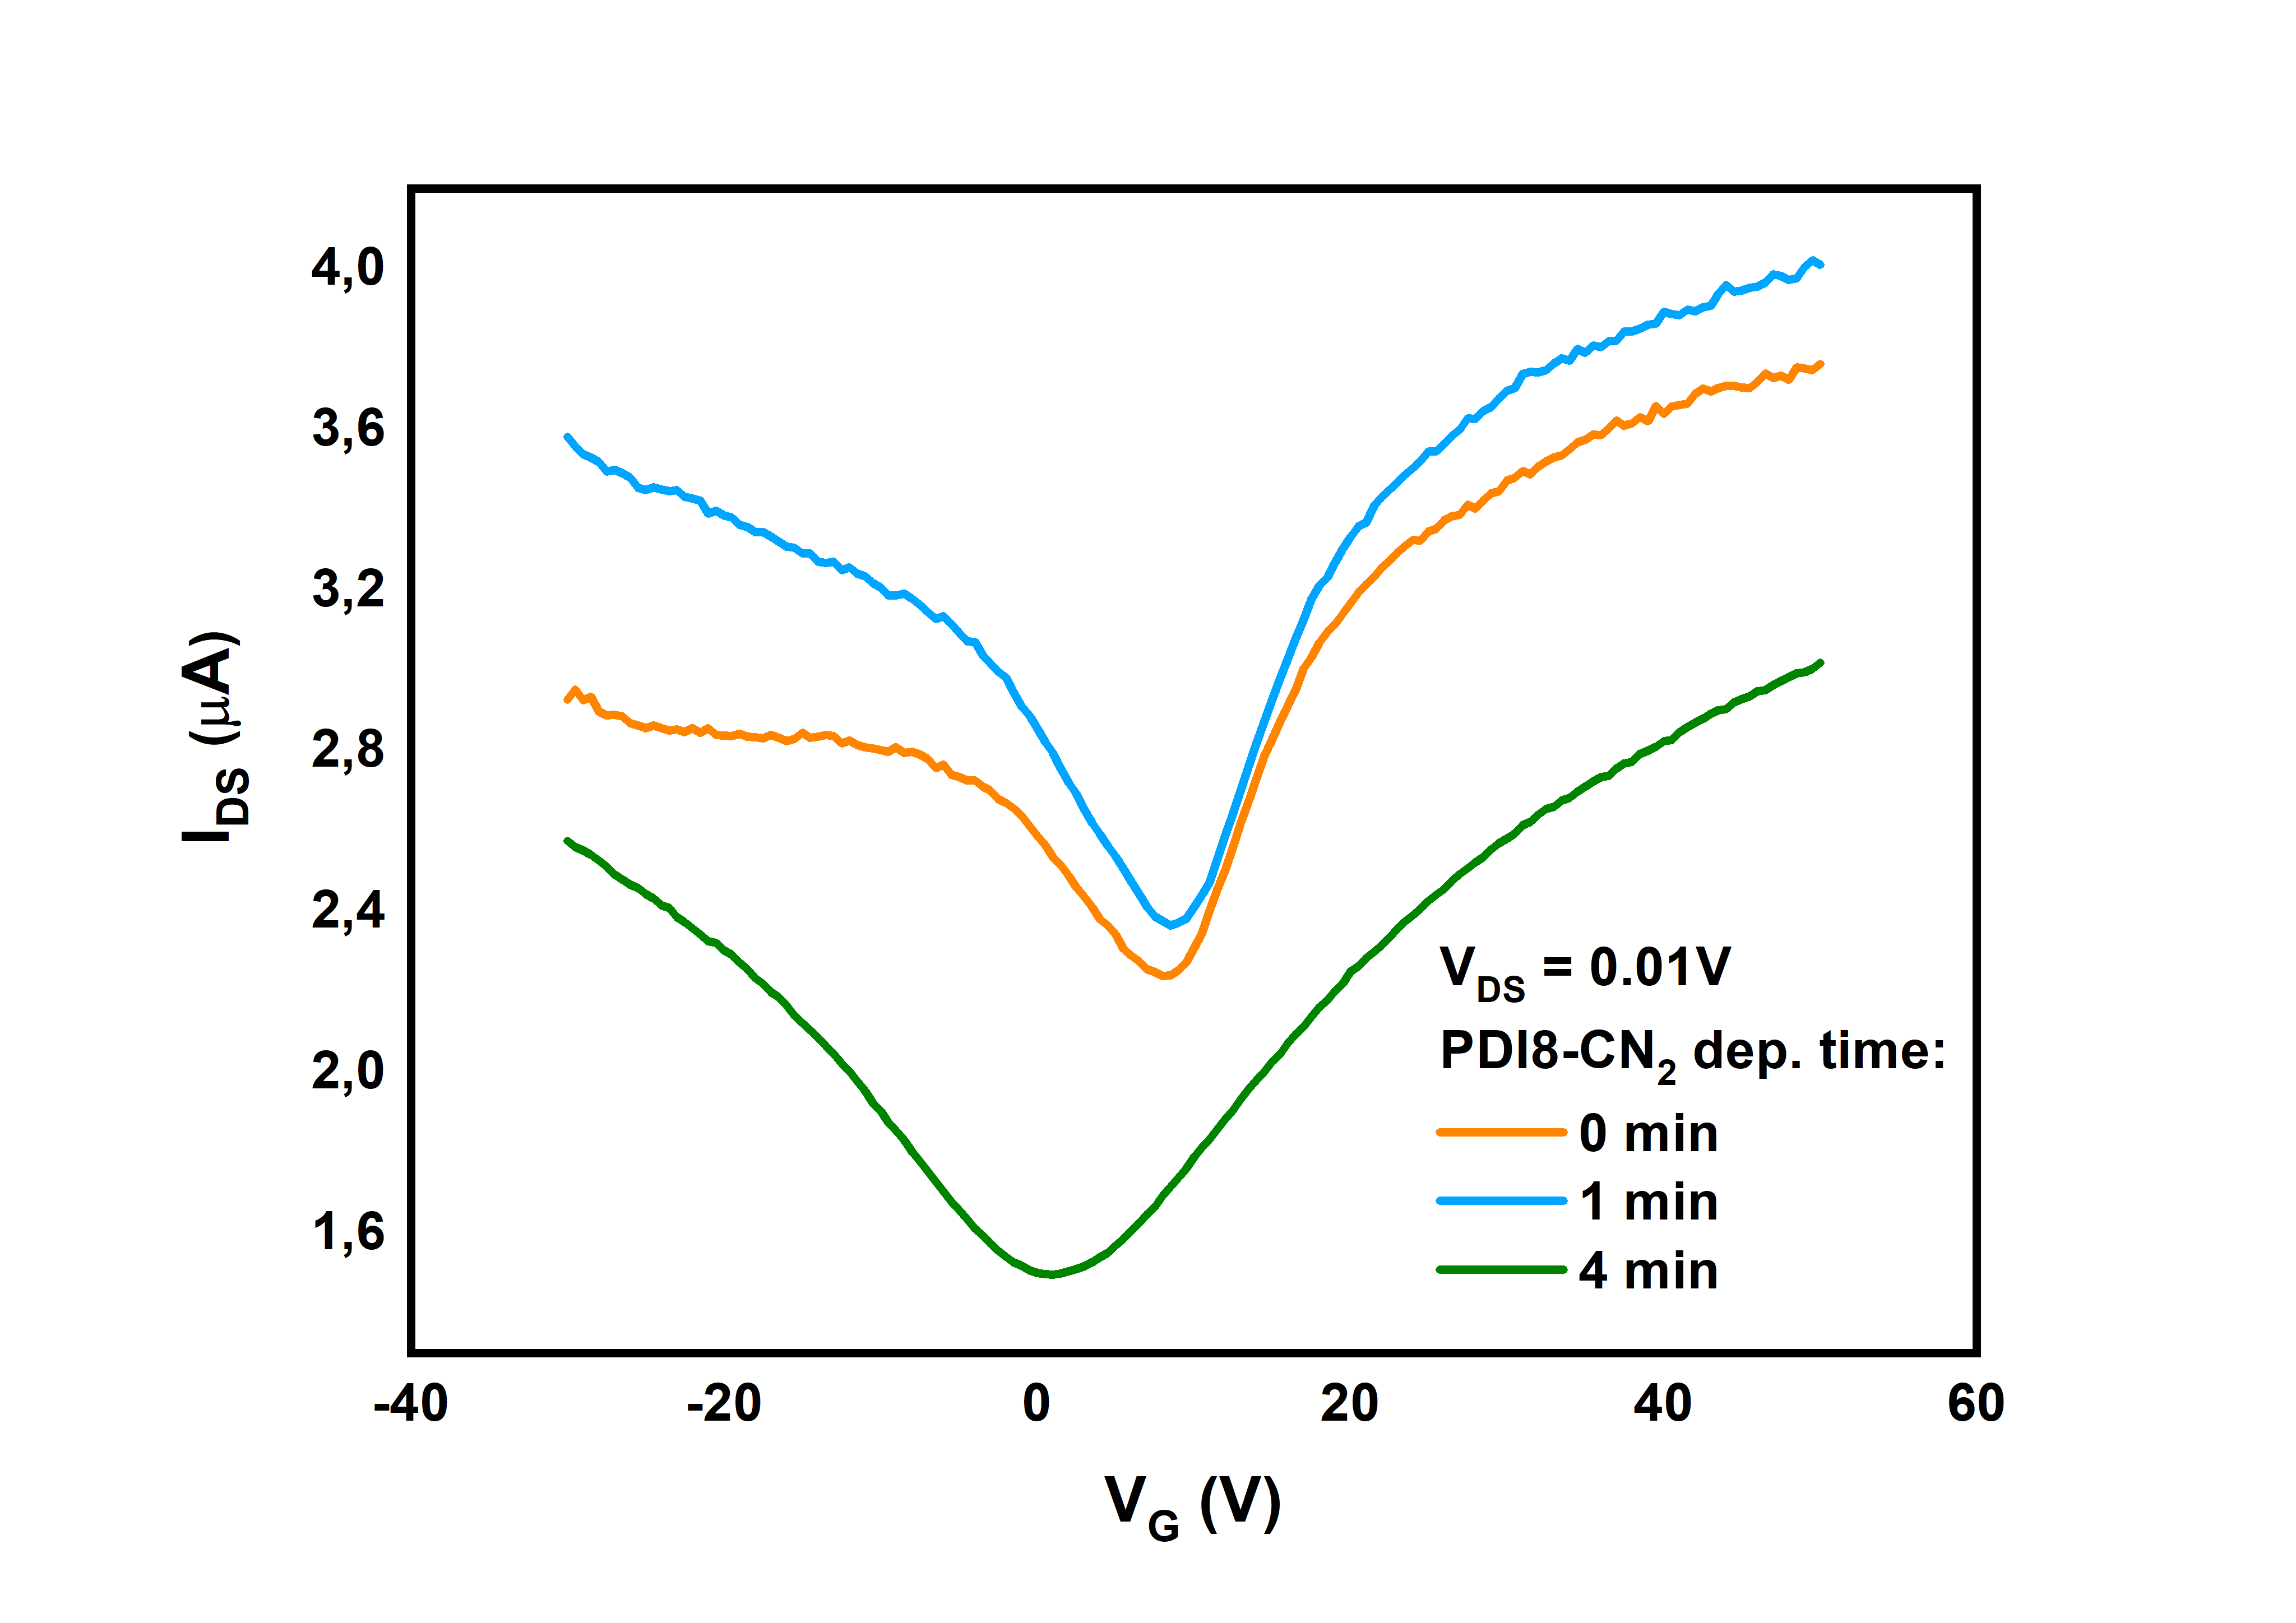
\includegraphics[width=0.9\textwidth]{./Figures/fig3}  
  \caption{Transconductance measurements of a graphene field-effect transistor at different PDI8-CN2 coverages of graphene. Red curve corresponds to clean graphene, blue curve corresponds to a coverage of 0.6 obtained by the PDI8-CN2 deposition of 1 minute. The green curve corresponds to the coverage obtained by PDI8-CN2 deposition of 3 minute. The corresponding morphologies are shown in Figures 1 and 2, respectively. }
  \label{fig:3}
\end{figure}

We observe transfer characteristics of GFET comprising clean graphene exhibiting charge-neutrality point at back-gate voltage of 8.5 V.  The position of CNP relative to the Dirac point (0 V) is consistent with $p$-type doping of graphene caused by the trap states on SiO$_{2}$ surface and chemical redox reaction occurring at the graphene/SiO$_{2}$ interface\cite{feng-2014,peng-2017,lafkioti-2010}.  In addition to the shift of the conductivity minimum we observe also a strong reduction in the slope of the transfer curve occurring at about 3.6 V, leading to a plateau of the drain current.  Such behavior is commonly present in GFETs with relatively short channels, where the role of the metallic contacts becomes important\cite{bartolomeo-2015,nouchi-2008,nouchi-2014}. Two principal mechanisms in GFET affect charge transport under ambient conditions. First is already mentioned doping of the channel with airborne species. The second is related to the graphene doping under metallic contacts\cite{farmer-2009,giovannetti-2008,lee-2008,mueller-2009}.  Several groups report the evidence that metallic contacts induce doping of the underlying graphene \cite{giovannetti-2008,mueller-2009,huard-2008}, and the amount of transferred charge depends on the difference of metallic work function and the work function of graphene.  Specifically, Au contacts used in our experiments cause p-type doping, according to the work by Giovanetti et al.\cite{giovannetti-2008}, causing a shift in Fermi level of 0.3 eV in the direction away from the vacuum level, across the Dirac point. In addition, changes in the interface charge density may be a consequence of Fermi-level depinning at the metal/graphene interface and is related to microscopic interface environment that is characterized by interdiffusion of metallic atoms and/or oxide interlayer\cite{nouchi-2008,nouchi-2014}. Since Fermi level at such interfaces is not pinned or only partially pinned\cite{dibartolomeo-2011}, the interface charge density may be affected by the applied gate voltage, which is not the case for the abrupt interfaces.  In the channel instead, we can calculate the position of the Fermi level relative to the Dirac point in graphene ($\Delta E$) from the measured position of CNP (Figure \ref{fig:3}), using the approach from Ref. \onlinecite{wang-2008}:
\begin{equation}
  \label{eq:1}
  \Delta E = \hbar v_{F}\sqrt{\pi\alpha|V_{g}-V_{D}}
\end{equation}

where $v_F=0.8\times10^6$ m/s, and $\alpha=7.2\times10^{14}$ cm$^{-2}$ V$^{-1}$. For the value $|V_g-V_D |=8.5$ V we obtain the position of the Fermi level to be 0.073 eV below the Dirac point. The channel structure can therefore be regarded as $p^{++}/p/p^{++}$. A consequence of such variation of charge density within the structure are deviations from the linear transfer lineshapes, which in extreme cases may result in curves may extreme with double dips\cite{nouchi-2014,nam-2012}, or in less extreme exhibiting an abrupt change in slope continuing to a plateau. 

\subsection{Transconductance - 1st coverage}
\label{sec:first}

At the PDI8-CN2 coverage of 0.6 the position of CNP is shifted slightly (for ~0.5 V)  to more positive voltages and the current at the CNP is slightly increased relative to the clean graphene.  More importantly, we note a less pronounced change in the slope of the transfer characteristics at negative gate voltages, compared to the one observed on clean graphene (red curve). The observed behavior of the transport properties can be understood in the context of rather complex morphology of PDI8-CN2 layers on graphene, and with is associated interaction of the PDI8-CN2 molecules with graphene. At the sub monolayer coverage of PDI8-CN2 the hole transport continues to proceed through the channel, relatively unhindered, electron transport, however is enhanced relative to clean graphene (cf. red and blue curve in Figure \ref{fig:3}). We have noted that the crossover in the transfer curve is related to the partial depinning of the Fermi level near the contacts. Due to the low density of states in graphene this interface environment may extend as far as 0.2 $\mu$m\cite{mueller-2009}. This is the area exposed to the flux of incoming PDI8-CN2 molecules during the organic layer growth and represents a place of nucleation of the PDI8-CN2 islands. The AFM results (Figure 1) show that at this coverage islands are formed in which the molecules are oriented face-on on the graphene surface. It has been shown\cite{su-2009} that molecules with large aromatic structures carrying surplus of negative charge are noncovalently bonded to graphene surface by $\pi-\pi$ interactions, which result in strong charge transfer at the interface. The additional charges that are brought to the interface by the organic molecules change the carrier concertation in graphene and change the position of the Fermi level, in the direction as to reduce the $p^{++}$ doping at the interface and therefore increase hole mobility in that region. The low position of LUMO in PDI8-CN2 (-4.3 eV)\cite{jones-2007} enables efficient electron transfer to graphene, reducing strong p-type doping levels near the Au contacts. Consequently, the cusp in the transfer curve is reduced.   As for the small shift of CNP relative to the clean graphene, it corresponds to to the change of position of Fermi level of only ~$3\times10^{-3}$ eV, indicating negligible charge transfer between PDI8-CN2 layer and graphene, which would affect its electronic properties. Interestingly, the 0.6 monolayer coverage agrees nicely with the 0.5 ML--0.7ML coverage of PDI8-CN2 at which the onset of  drain-source current is observed in PDI8-CN2-based organic thin film transistors\cite{liscio-2013}. 

\subsection{Transconductance of the complete PDIF9 layer}
\label{sec:complete}

At the complete coverage of PDI8-CN2 (green curve) the line shape of the transfer characteristics typical for graphene remains qualitatively the same (green curve, Figure \ref{fig:3}).  The position of CNP exhibits a strong negative shift ($V_g=0.5$ V) and an important reduction of the drain current relative to the clean graphene. Importantly, the transfer curve appears almost symmetric.  As the AFM data show the second layer comprises PDI8-CN2 molecules oriented upright with their aromatic cores facing each other, facilitating thereby intermolecular overlap of the $\pi$-states and minimizing trap density.  Strong shift of CNP indicates that strong electron doping from the second layer of PDI8-CN2 to  graphene occurs. As the PDI8-CN2 coverage increases, charge transport in the channel is strongly affected
These qualitative assertions were confirmed also numerically by modeling the resistance determined from the transfer characteristic. 

\subsection{Model}
\label{sec:model}

The resistance plots calculated from the data used to plot Figure \ref{fig:4}.  Are shown in modeled the transfer characteristics were modeled under the following assumptions. The gate voltage is a sum of contributions due to the quantum capacitance, given by the position of the Fermi level  ($E_F$) in graphene and the  electrostatic potential difference between the graphene layer and the gate contact, given by $n\cdot e/C_{ox}$ with $C_{ox}$ capacitance of the gate dielectric and $n$  charge carrier concentration\cite{sze-2006}[26].  However, the gate capacitance $C_{ox}=(\epsilon_0\epsilon)/d_{ox} =1.2\times10^8$ F cm$^{-2}$, with dielectric constant of SiO$_{2}$  $\epsilon \approx 4$ and $d_{ox}=$300 nm.  Considering the typical charge carrier densities on the order of $10^{13}$ cm$^{-2}$ the potential difference accommodated by the bottom gate contact amounts ot 100 V, which is considerably larger than the Fermi level shift in graphene.  Quantum capacitance in the case of bottom gate contact may therefore be safely neglected\cite{das-2008}. The drain current was  calculated as:
\begin{equation}
  \label{eq:2}
  I_{D}=\frac{W}{L}\mu n e)V_{D}- 2I_{D}R_{C}
\end{equation}

\begin{figure}[htb]
  \centering
   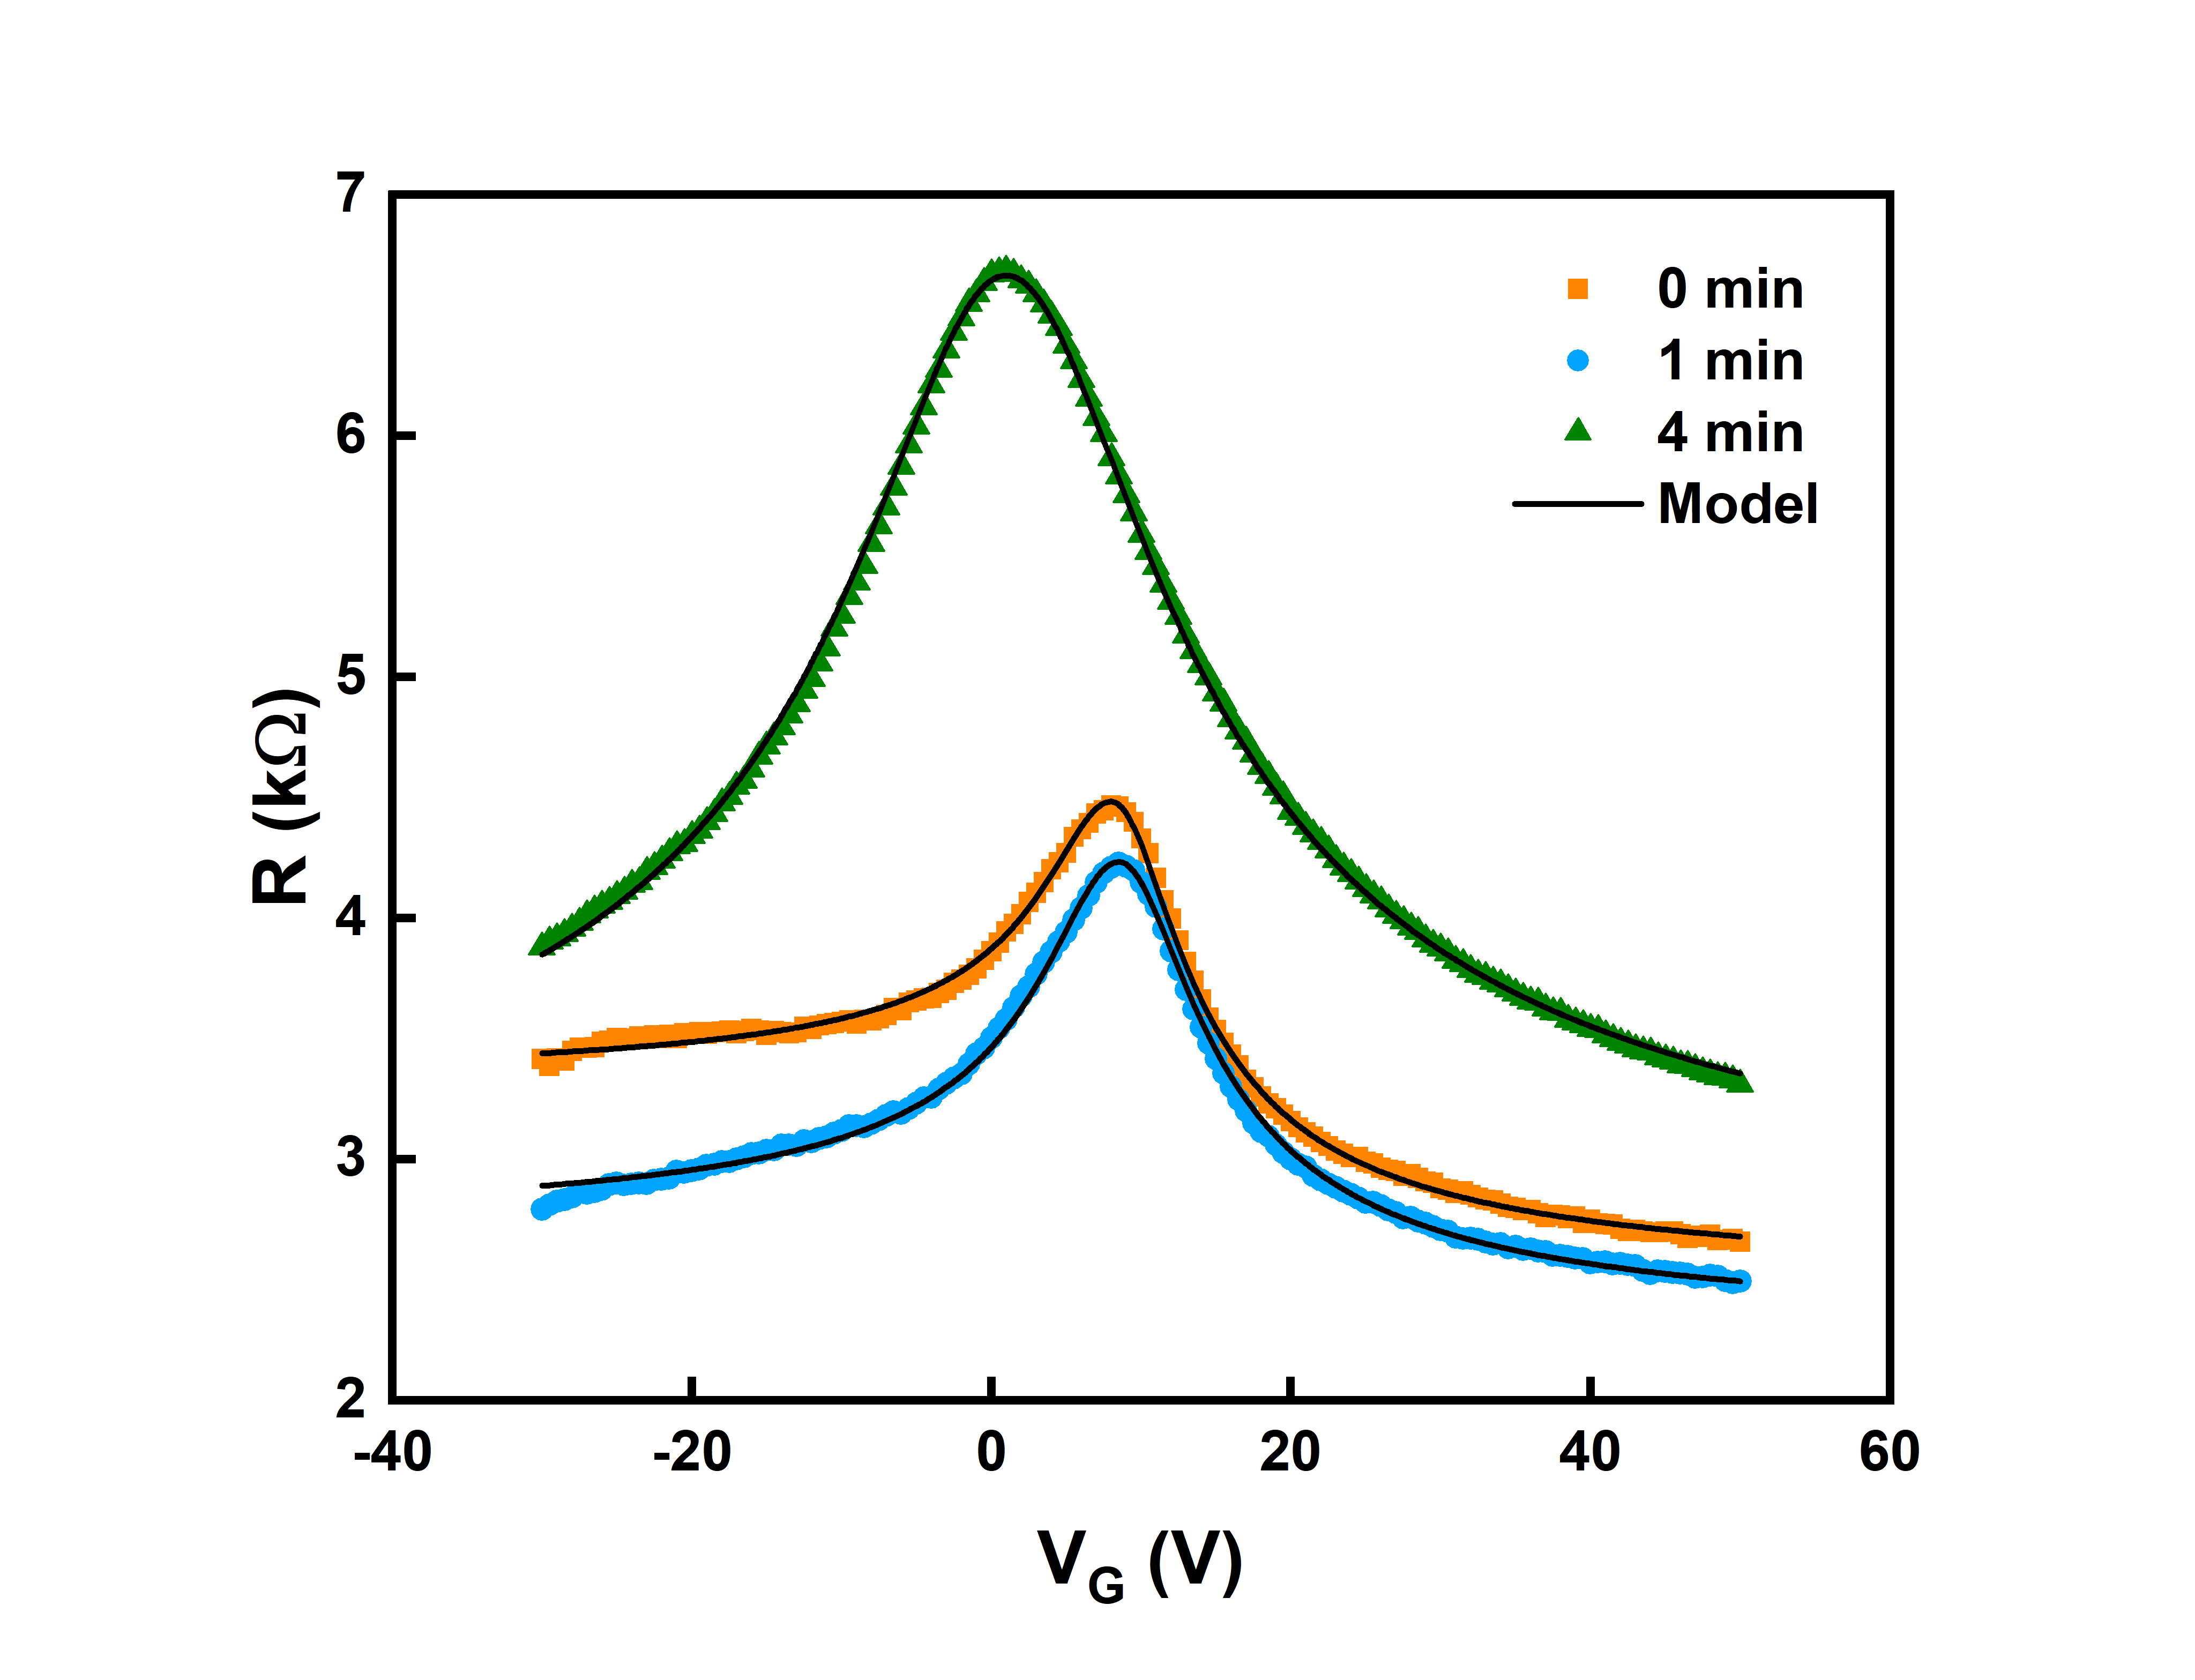
\includegraphics[width=0.9\textwidth]{./Figures/fig4}  
  \caption{Resistance calculated from the data presented in Figure 3 (symbols). Solid lines represent least-squares fits based on the Equation \ref{eq:5}.}
  \label{fig:4}
\end{figure}

\noindent With $W$ and $L$ channel width and length respectively, $R_{C}$ the resistance of both metallic contacts, $\mu$ charge carrier mobility and n their concentration. Given by:
\begin{equation}
  \label{eq:3}
  n_{s}=\sqrt{n_{o}^{2}+n^{2}(V_{g})}
\end{equation}

and 
\begin{equation}
  \label{eq:4}
  n(V_{g})= \frac{C_{ox}}{e}(V_{D}- V_{CNP})
\end{equation}


\noindent With $V_{CNP}$ the gate voltage of the charge-neutrality point\cite{xia-2010}. Since the total resistance of the structure is the resistance of the channel plus the resistance of the contacts:
\begin{equation}
  \label{eq:5}
  R_{tot} = \frac{V_{D}}{I_{D}} = \frac{L}{W\mu e\sqrt{n_{0}^{2}+n^{2}(V_{g})}} +2 R_{c}
\end{equation}


\noindent The results of the least-square fitting to a function presented in Equation 1 are shown by solid lines in Figure 4. The fitting parameters were the contact resistivity, mobility and $n_0$ and $n(V_g)$.  The results of fitting for the three cases are summarised in Table 1.
\noindent \begin{table}[h]
  \centering
  \begin{tabular}{|l|r|r|r|r|r|r|} \hline%
   & $n_{0}$ (cm$^{-2}$ )& $R_{c}^{h}(\Omega$) & $R_{c}^{e}(\Omega)$ & $\mu_{h}$ (cm$^{2}$/Vs) & $\mu_{e}$ (cm$^{2}$/Vs) & $V_{D}(V) $  \\ \hline%
    Clean gr. & 3.33$\times 10^{11}$ & 3303 & 2469 & 26920 & 15772 & 8 \\
    70\% cov. &3.71$\times 10^{11}$ & 2694 & 2262 & 18537 & 14474 & 8.5 \\
     100\% cov. &7.42$\times 10^{11}$ & 2632 & 2548 & 3543 & 3471 & 1 \\ \hline
    
  \end{tabular}
  \caption{The results of fitting of resistance crves shown in Figure \ref{fig:3}. See  text for the explantaion of the parameters.}
  \label{tab:1}
\end{table}

\subsection{Interpretation of the Fitting Results}
\label{sec:interp}

Firstly, we focus on the initial charge carrier density $n_0$, which stems from the impurities residing either at the graphene interface or within the gate dielectric. On clean graphene we obtained a value of 3.33$\times 10^{11}$ cm$^{-2}$, which may be considered a ``clean'' sample for long-range scattering.  As the coverage of PDI8-CN2 is increased to 0.7 $n_0$ exhibits only a slight increase to 3.71$\times 10^{11}$ cm$^{-2}$, but almost doubles at full coverage ($n_{0}=7.42\times 10^{11}$ cm$^{-2}$).
In order to explain the observed behavior, we have to consider the dependence of the electronic structure of organic thin layers on the molecular orientation.  Anisotropic behavior of charge transport properties of organic thin films are known for some time now\cite{sundar-2004}. Less common are detailed studies of the dependence of the position of the electron energy levels at different molecular orientation. This is particularly true for $n$-type OSs on graphene. Zhang et al.\cite{zhang-2016d} have performed a systematic photoelectron spectroscopy study coupled to density functional theory (DFT) -based calculations of electrostatic potential surfaces of several organic semiconductors including n-type. Their findings demonstrate energy shifts of the electronic structures as high as 0.54 eV between the layers with the molecules oriented upright and flat-lying molecules.  Crucial for such difference is the existence of the dipole (and quadrupole) electric field arising at different moieties of the molecules. For example, in the case of pyrrolo[3,4-c]pyrrole-1,4-dione (DPP)  the calculations show a surface electric dipole due to the electron-withdrawing carbonyl and imine groups pointing  away from the surface when the molecules are oriented upright (shorter molecular axis perpendicular to the surface). On the other hand flat-lying DPP molecules exhibit a quadrupole moment that points towards the surface. Consequently, the energy of HOMO is closer to the vacuum level in the case of flat-lying molecules relative to upright oriented molecules.  

Qualitatively, we can apply these arguments also for the case of PDI8-CN2 molecules. In the absence of available calculations of the electrostatic potential over the PDI8-CN2 molecule, we can speculate that the imide groups provide an electric dipole that points away from the surface and therefore increases electron binding energy. On the other hand DFT calculations of the electrostatic potential of the perylene core by Geng et al.\cite{geng-2012} show an abundance of negative charge inside the core, implying  that the $\pi$-electron system above the molecule represents an electron-deficient region, resulting in a surface dipole pointing towards the surface. Consequently, the electron binding energy in the layer of flat-lying molecules is lower relative to the upright oriented molecules.  In the case of 4 minute exposure the energy band alignment in the resulting structure corresponds to a type-II heterostructure with graphene and the intermediate layer of flat-lying molecules with energy band structure shifted closer to the vaccum level than the outer layer.  The direction of the dipole electric field of the first molecular layer precludes appreciable induction of the electric charge due to the back-gate, and slightly shifts CNP point towards the positive gate voltages. As the second molecular layer is completed, the resulting dipole electric field -- directed away from the surface favors electron accumulation at the graphene interface resulting in a strong shift of the CNP in the negative direction.  The molecular density of the second layer is considerably higher with perylene core interplanar of $< 0.34$ nm, which results in higher dipole electric field intensity than in  case of the layer comprising the flat-lying molecules.

Coupled to the change in the position of CNP is also an increase in the overall resistance of the structure. This is because for the OS layers the metallic contacts are of the  bottom-contact type, and charge transport occurs in parallel through graphene and the second layer of PDI8-CN8, in which $\pi$-stacking provides more favorable charge transporting lane than the flat-lying molecules. Overall resistance is therefore net resistance between graphene and PDI8-CN2. Interestingly the asymmetry in contact resistance for holes (R$_{h}$) and  electrons  (R$_{e}$) on clean graphene as obtained from the model is quite appreciable and reflects the qualitative arguments given above.  On fully covered graphene, when the charge transport proceeds also over PDI8-CN2 layer for which the contacts are of the bottom-type this asymmetry almost vanishes (R$_{e}$=2632 $\Omega$, vs. R$_{h}=2548\ \Omega$).  Coupled to the doping structure of the channel discussed above is also asymmetry in hole mobility  ($\mu_{h}= 26920$ cm$^{2}$/Vs ) and electron mobility ($\mu_{h}= 15772$ cm$^{2}$/Vs) on clean graphene. As the PDI8-CN2 layer is completed the mobility is drastically reduced relative to the clean graphene.  This argues for the opening of the charge transport venue through the second layer of $\pi-\pi$ molecular array. Transport is ambipolar and characterized by charge carrier mobility values that are unprecedented for an OS-graphene system.  

\section{Conclusions}
\label{sec:conc}

In conclusion, our charge transport experiments of the graphene/PDI8-CN2 heterostructures coupled with numerical modeling of the resistivity data demonstrate a crucial role that molecular orientation on graphene has on charge carrier transport properties of graphene field effect transistors with organic semiconductor channels.  We have shown that under precisely controlled growth conditions PDI8-CN2 form a first continuous monolayer characterized by exclusively flat-lying molecules.  Due to the orientation of the surface multipolar electric field associated with such orientation of the molecules their effect on the doping levels  of  the underlying graphene is only minor, if anything it slightly increases p-type doping of graphene. The growth mode of PDI8-CN2 is peculiar in the sense that it proceeds in a layer-by-layer fashion also in the second layer. However, the molecules in the second layer are oriented in a upright fashion, exposing the dipole electric field that stems mostly from electron withdrawing groups in such a way as to increase n-type doping of graphene, as manifested by the shift of the Fermi  level almost to the Dirac point.  Coupled to this is also opening of another transport channel via the PDI8-CN2 topmost layer, which maintains extremely high mobility of the OS-graphene system.

\section*{Acknowledgments}


This work was supported in part by the Slovenian Research Agency under research program P1-0055.  V. T.  acknowledges SRA's support under the Young Researcher's scheme.   


\bibliography{literaturaMar2020}


\end{document}

%%% Local Variables:
%%% mode: latex
%%% TeX-master: t
%%% End:
